307. На схеме изображён пустой стальной кубик со стороной 1 метр. На каждой его грани нарисовали 25 одинаковых квадратиков и просверлили три дырки как показано на рисунке. Кубик можно ставить на другие грани, но нельзя дыркой вниз. Какое наибольшее количество литров воды можно налить в этот кубик? Напомним, что литр --- это дециметр кубический.
\begin{figure}[ht!]
\center{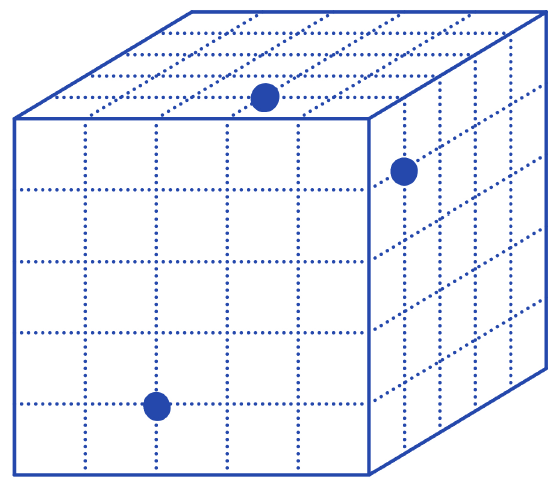
\includegraphics[scale=0.35]{kukub.png}}
\end{figure}\\
